\documentclass[tikz,convert={outfile=\jobname.svg}]{standalone}
\usetikzlibrary{positioning,fit,calc}
\usepackage{fontspec}
\setmainfont{Gentium Plus}
\begin{document}

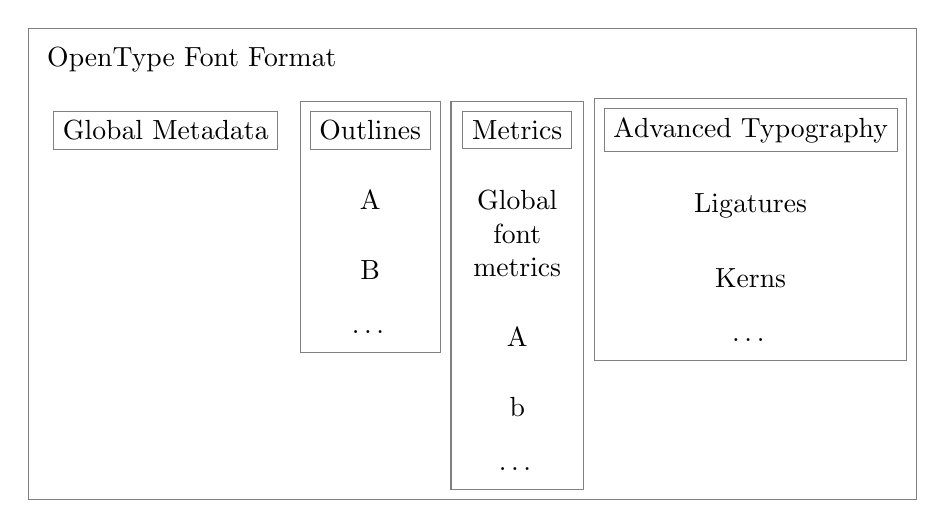
\begin{tikzpicture}[
  node distance=4mm,
  typetag/.style={rectangle, draw=black!50, anchor=west}
]
  \node (toplevel) { OpenType Font Format };

  \node (gm) [below=of toplevel.west, typetag, yshift=-5mm, xshift=2mm] { Global Metadata };

  \node (outlines) [right=of gm, typetag] { Outlines };
  \node (outa) [below=of outlines] { A};
  \node (outb) [below=of outa] { B };
  \node (outdots) [below=of outb] { \dots };
  \node (outbox) [draw=black!50, fit={(outlines) (outa) (outb) (outdots)}] {};

  \node (metrics) [right=of outlines, typetag] { Metrics };
  \node (gmetrics) [below=of metrics,text width=12mm,align=center] { Global font metrics};
  \node (metricsa) [below=of gmetrics] { A };
  \node (metricsb) [below=of metricsa] { b };
  \node (metricsdots) [below=of metricsb] { \dots };
  \node (metricsbox) [draw=black!50, fit={(metrics) (gmetrics) (metricsa) (metricsdots)}] {};

  \node (otmagic) [right=of metrics, typetag] { Advanced Typography };
  \node (ligs) [below=of otmagic] { Ligatures };
  \node (kerns) [below=of ligs] { Kerns };
  \node (otdots) [below=of kerns] { \dots };
  \node (otbox) [draw=black!50, fit={(otmagic) (ligs) (kerns) (otdots)}] {};

  \node [draw=black!50, fit={(toplevel) (gm) (outbox) (metricsbox) (otbox)}] {};
\end{tikzpicture}
\end{document}